\documentclass[spanish,a4paper,12pt,oneside]{extreport}

\usepackage[dvips]{graphicx}
\usepackage[dvips]{epsfig}
\usepackage[utf8]{inputenc}
\usepackage[spanish]{babel}
\usepackage{alltt}

\usepackage[ruled,vlined,commentsnumbered,linesnumbered,inoutnumbered,titlenotnumbered,noend]{algorithm2e}
\SetKwRepeat{Do}{do}{while}

\usepackage{multirow}
\usepackage{array} 
\usepackage{amsfonts}
\usepackage{amsmath}
\usepackage{bigstrut}
\usepackage{booktabs}
\usepackage{caption}
\usepackage{chngpage}
\usepackage{float}
\usepackage{enumitem,lipsum}
\usepackage{graphicx}
\usepackage{lscape}
\usepackage{microtype}
\usepackage{natbib}
\usepackage{pdflscape}
\usepackage{rotating}
\usepackage{subcaption}
\usepackage{ctable}
\usepackage{hyperref}
\usepackage{enumerate}
\usepackage{gensymb}
\usepackage{eurosym}
\usepackage{xcolor}
\usepackage{tabu}

\usepackage{lineno}
%\\linenumbers
%\setlength\linenumbersep{5pt}
%\renewcommand\linenumberfont{\normalfont\tiny\sffamily\color{gray}}

\usepackage[top=2cm, bottom=2cm, left=2cm, right=2cm]{geometry}

\newenvironment{sourcecode}
{\begin{list}{}{\setlength{\leftmargin}{1em}}\item\scriptsize\bfseries}
{\end{list}}

\newenvironment{littlesourcecode}
{\begin{list}{}{\setlength{\leftmargin}{1em}}\item\tiny\bfseries}
{\end{list}}

\newenvironment{summary}
{\par\noindent\begin{center}\textbf{Abstract}\end{center}\begin{itshape}\par\noindent}
{\end{itshape}}

\newenvironment{keywords}
{\begin{list}{}{\setlength{\leftmargin}{1em}}\item[\hskip\labelsep \bfseries Keywords:]}
{\end{list}}

\newenvironment{palabrasClave}
{\begin{list}{}{\setlength{\leftmargin}{1em}}\item[\hskip\labelsep \bfseries Palabras clave:]}
{\end{list}}

\usepackage{bera}% optional: just to have a nice mono-spaced font
\usepackage{listings}
\usepackage{xcolor}

\colorlet{punct}{red!60!black}
\definecolor{background}{HTML}{EEEEEE}
\definecolor{delim}{RGB}{20,105,176}
\colorlet{numb}{magenta!60!black}

\lstdefinelanguage{json}{
    basicstyle=\normalfont\ttfamily,
    numbers=left,
    numberstyle=\scriptsize,
    stepnumber=1,
    numbersep=8pt,
    showstringspaces=false,
    breaklines=true,
    frame=lines,
    backgroundcolor=\color{background},
    literate=
     *{0}{{{\color{numb}0}}}{1}
      {1}{{{\color{numb}1}}}{1}
      {2}{{{\color{numb}2}}}{1}
      {3}{{{\color{numb}3}}}{1}
      {4}{{{\color{numb}4}}}{1}
      {5}{{{\color{numb}5}}}{1}
      {6}{{{\color{numb}6}}}{1}
      {7}{{{\color{numb}7}}}{1}
      {8}{{{\color{numb}8}}}{1}
      {9}{{{\color{numb}9}}}{1}
      {:}{{{\color{punct}{:}}}}{1}
      {,}{{{\color{punct}{,}}}}{1}
      {\{}{{{\color{delim}{\{}}}}{1}
      {\}}{{{\color{delim}{\}}}}}{1}
      {[}{{{\color{delim}{[}}}}{1}
      {]}{{{\color{delim}{]}}}}{1},
}

\begin{document}

\renewcommand\listtablename{Índice de Tablas}    
\renewcommand\listfigurename{Índice de Figuras}    

%%%%%%%%%%%%%%%%%%%%%%%%%%%%%%%%%%%%%%%%%%%%%%%%%%%%%%%%%%%%%%%%%%%%%%%%%%%%%%%
% First Page
%%%%%%%%%%%%%%%%%%%%%%%%%%%%%%%%%%%%%%%%%%%%%%%%%%%%%%%%%%%%%%%%%%%%%%%%%%%%%%%
\pagestyle{empty}
\thispagestyle{empty}


\newcommand{\HRule}{\rule{\linewidth}{1mm}}
\setlength{\parindent}{0mm}
\setlength{\parskip}{0mm}

\vspace*{\stretch{0.5}}

\begin{center}

\includegraphics[scale=0.8]{images/escuela-ingenieria-tecnologia-original}\\[10mm]
{\Huge Informe de Prácticas}
\end{center}

\HRule
\begin{flushright}
        {\Huge Robótica Computacional} \\[2.5mm]
        {\Large \textit{Grado en Ingeniería Informática}} \\[5mm]
        {\Large José Ramón Morera Campos} \\[5mm]


\end{flushright}
\HRule
\vspace*{\stretch{2}}
\begin{center}
  \Large La Laguna, \today
\end{center}

\setlength{\parindent}{5mm}

%%%%%%%%%%%%%%%%%%%%%%%%%%%%%%%%%%%%%%%%%%%%%%%%%%%%%%%%
\newpage{\pagestyle{empty}}
\thispagestyle{empty}

%%%%%%%%%%%%%%%%%%%%%%%%%%%%%%%%%%%%%%%%%%%%%%%%%%%%%%%%%
\pagestyle{myheadings} %my head defined by markboth or markright
% No funciona bien \markboth sin "twoside" en \documentclass, pero al
% ponerlo se dan un monton de errores de underfull \vbox, con lo que no se
% ha puesto.


%%Aqui debería poner el nombre del proyecto pero, como es muy grande no cabe y se ve feo en el PDF
\markboth{xxxxx}{}

%%%%%%%%%%%%%%%%%%%%%%%%%%%%%%%%%%%%%%%%%%%%%%%%%%%%%%%%%
%Numeracion en romanos
\renewcommand{\thepage}{\roman{page}}
\setcounter{page}{1}
\pagestyle{plain} 

%%%%%%%%%%%%%%%%%%%%%%%%%%%%%%%%%%%%%%%%%%%%%%%%%%%%%%%%%

\tableofcontents

%%%%%%%%%%%%%%%%%%%%%%%%%%%%%%%%%%%%%%%%%%%%%%%%%%%%%%%%%
\newpage
\pagestyle{empty}

\listoffigures

%%%%%%%%%%%%%%%%%%%%%%%%%%%%%%%%%%%%%%%%%%%%%%%%%%%%%%%%%%%%%%%%%%%%%%%%%%%%%%%
\newpage{\pagestyle{empty}}

%%%%%%%%%%%%%%%%%%%%%%%%%%%%%%%%%%%%%%%%%%%%%%%%%%%%%%%%%%%%%%%%%%%%%%%%%%%%%%%
\newpage
\thispagestyle{empty}

%Numeracion a partir del capitulo I
\renewcommand{\thepage}{\arabic{page}}
\setcounter{page}{1}
\pagestyle{plain}

\chapter{\LARGE Introducción}
\label{chapter:intro}


En este informe se analizan las cuatro prácticas realizadas a lo largo de la asignatura de Robótica Computacional. 

\bigskip Se estudia el comportamiento de los programas realizados, mostrando ejemplos con diversas configuraciones de parámetros. Adicionalmente, se explican las modificaciones realizadas, así como otras propuestas de mejora. 

\bigskip Finalmente, para cada prácitca se exponen unas breves conclusiones sobre los resultados obtenidos. Dichas conclusiones se exponen en ingles, siguiendo los requisitos del informe.


%%%%%%%%%%%%%%%%%%%%%%%%%%%%%%%%%%%%%%%%%%%%%%%%%%%%%%%%%%%%%%%%%%%%%%%%%%%%%%%
\newpage{\pagestyle{empty}}
\thispagestyle{empty}

\chapter{\LARGE Cinemática Directa}
\label{chapter:dos}

En esta práctica se calcula la cinemática directa para manipuladores tridimensionales. 
Se modifica la morfología del robot indicando la longitud de los elementos rígidos, así como la existencia de articulaciones de revolución o prismáticas.
Al ejecutar el script se indican los valores de las variables articulares.

\section{Código Implementado}
El script proporcionado contiene todo el código necesario para calcular la cinemática directa y visualizar los manipuladores. 
Solamente se deben modificar ciertos parámetros para adaptar el script a la morfología del robot:
\begin{itemize}
   \item \texttt{nvar} Número de variables que se introduciran al ejecutar el programa, correspondientes a las variables articulares.
   \item \texttt{Parámetros de Denavit–Hartenberg} son 4 vectores, uno para cada parámetro. El tamaño del vector se corresponde al número de articulaciones.
   \item \texttt{Orígenes para cada articulación} un vector con las coordenadas homogéneas de cada articulación.
   \item \texttt{Matrices T} son matrices que permiten realizar la transformación de un sistema de coordenadas a otro.
   Las matrices entre sistemas consecutivos son triviales, y se construyen con sus parámetros de Denavit–Hartenberg.
   Las matrices que describen la transformación entre sistemas no consecutivos se obtienen multiplicando las matrices de transformación de los sistemas intermedios.
   Por ejemplo, la matriz T02, que transforma el sistema de coordenadas 0 al 2, se obtiene realizando el producto de las matrices T01 y T12.
   \item \texttt{Coordenadas de cada articulación} se calcula el origen de coordenadas del sistema de cada articulación mediante el producto punto a punto de la matriz de transformación T0X y el origen de coordenadas oXX.
   \item \texttt{Visualización del robot} se deben modificar las instrucciones de visualización para adaptarlas a la morfología del robot, incluyendo los origenes de coordenadas calculados que se quieren visualizar.
\end{itemize}
En la figura~\ref{chapter:intro2} se muestra el fragmento del script que se debe modificar.
\begin{figure}[htb]
   \centering
   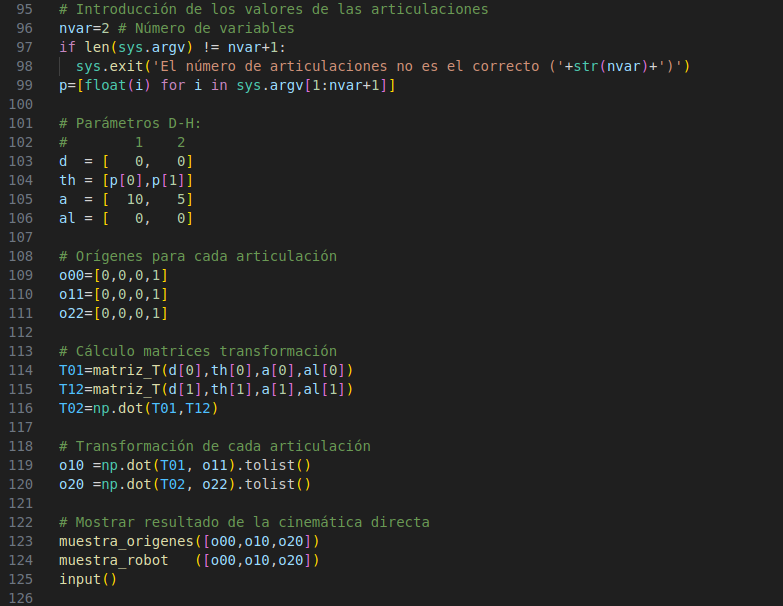
\includegraphics[width=1\linewidth]{images/cin_dir_1.png}
   \caption{Porción del código que se debe modificar para cada manipulador}
   \label{chapter:intro2}
\end{figure}
%%%%%%%%%%%%%%%%%%%%%%%%%%%%%%%%%%%%%%%%%%%%%%%%%%%%%%%%%%%%%
\section{Ejemplo}
Se emplea el Manipulador 3 de entre los propuestos para visualizar la cinemática directa. Se ha elegido puesto que tiene suficiente complejidad para ilustrar correctamente la práctica, pero sin ser excesiva.
\subsection{Código}

\subsection{Ejecución}

\section{Mejoras}
En esta práctica no se han implementado mejoras, pero se proponen algunas que podrían ser interesantes.
\begin{itemize}
   \item \texttt{Lectura de JSON} se podría implementar la lectura de la morfología del robot desde un ficheor JSON, evitando tener que modificar el script para cada manipulador.
   \item \texttt{Modificación de los parámetros en tiempo real} Sería de gran utilidad poder modificar las variables articulares mientras se visualiza el manipulador, para poder estudiar fácilmente cómo lo afectan.
\end{itemize}

\section{Conclusions}
We have studied the forward kinematics of a 3D manipulator. We have seen that we can characterize any manipulator by its Denavit-Hartenberg parameters, and that it is easy to calculate the coordinates of each joint. 
We have also seen that the visualization of the manipulator is very useful to understand its behavior and to check that the calculations made to obtain the parameters are correct.

\bigskip Although the script provided is very useful, it has room for improvements. Also, we still have to manually calculate the Denavit-Hartenberg parameters, which can be a tedious task for complex manipulators.

%%%%%%%%%%%%%%%%%%%%%%%%%%%%%%%%%%%%%%%%%%%%%%%%%%%%%%%%%%%%%%%%%%%%%%%%%%%%%%%
\newpage{\pagestyle{empty}}
\thispagestyle{empty}

\chapter{\LARGE Cinemática Inversa}
\label{chapter:tres}

En esta práctica se calcula la cinemática inversa para manipuladores bidimensionales. Es decir, se obtienen las variables articulares necesarias para alcanzar un punto objetivo en el plano. Para ello, se emplea el algoritmo iterativo \textit{Cyclic Coordinate Descent} (CCD).

\bigskip Se caracteriza el robot mediante sus articulaciones, prismáticas o de revolución, y sus parámetros de Denavit-Hartenberg theta y a (al encontrarnos en 2D solo hay 2 parámetros).
Al ejecutar el script se indica las coordenadas del punto objetivo para el extremo del robot, y se obtienen las variables articulares necesarias para alcanzar dicho punto.

\section{Código Implementado}

\subsection{Análisis}
El script proporcionado contiene muchas de las funciones necesarias, sin embargo, se deben implementar varias funciones para poder calcular la cinemática inversa. Principalmente, se debe implementar la lógica del CCD. Se realiza un cálculo para cada articulación desde el extremo final (EF) hasta el origen del robot, actualizando su valor y recalculando la cinemática directa. Al finalizar, se comprueba la distancia al punto objetivo, si es menor a la tolerancia indicada (umbral de convergencia epsilon), se finaliza. En caso contrario, se itera hasta conseguir una aproximación tolerable, o que se detecte la imposibilidad de convergencia.
\begin{itemize}
   \item \texttt{Detección del tipo de articulación} se distingue entre articulaciones prismáticas y de revolución.
   \item \texttt{Cálculo de las articulaciones prismáticas} Para calcular la distancia que se incrementa o decrementa la articulación, se calcula la distancia entre el extremo del robot y el punto objetivo, proyectada sobre la recta de movimiento de la articulación prismática. Esto se consigue realizando el producto del vector unitario $\vec{u}$, que representa la dirección de la variable prismática, y el vector $\vec{v}$, que une el extremo del robot y el punto objetivo. El vector $\vec{u}$ se obtiene sumando los ángulos de todas las articulaciones previas a la actual, y calculando el seno y coseno del resultado. 
   \item \texttt{Cálculo de las articulaciones de revolución} se calcula el ángulo en el que se debe modificar la articulación calculando la diferencia entre el vector $\vec{v}$, que une la articulación de rotación y el punto extremo EF, y el vector $\vec{w}$, que une la articulación de rotación y el punto objetivo. Para ello, se normalizan ambos vectores y se calcula la diferencia entre sus arcotargentes. En la práctica, se emplea la función \textit{math.atan2} ya que se encarga de realizar las comprobaciones necesarias de cuadrantes.
   \item \texttt{Corrección de ángulo de rotación} se corrige el ángulo calculado para que se encuentre en el rango $[-\pi, \pi]$.
   \item \texttt{Límites} se implementan límites inferiores y superiores para cada articulación. En caso de que el nuevo valor de las variables articulares este por debajo, se emplea el límite inferior, y si está por encima, el superior.
\end {itemize}

En las figuras~\ref{chapter:code_ccd1} y ~\ref{chapter:code_ccd2} se muestra el código implementado para el CCD.
\begin{figure}[htb]
   \centering
   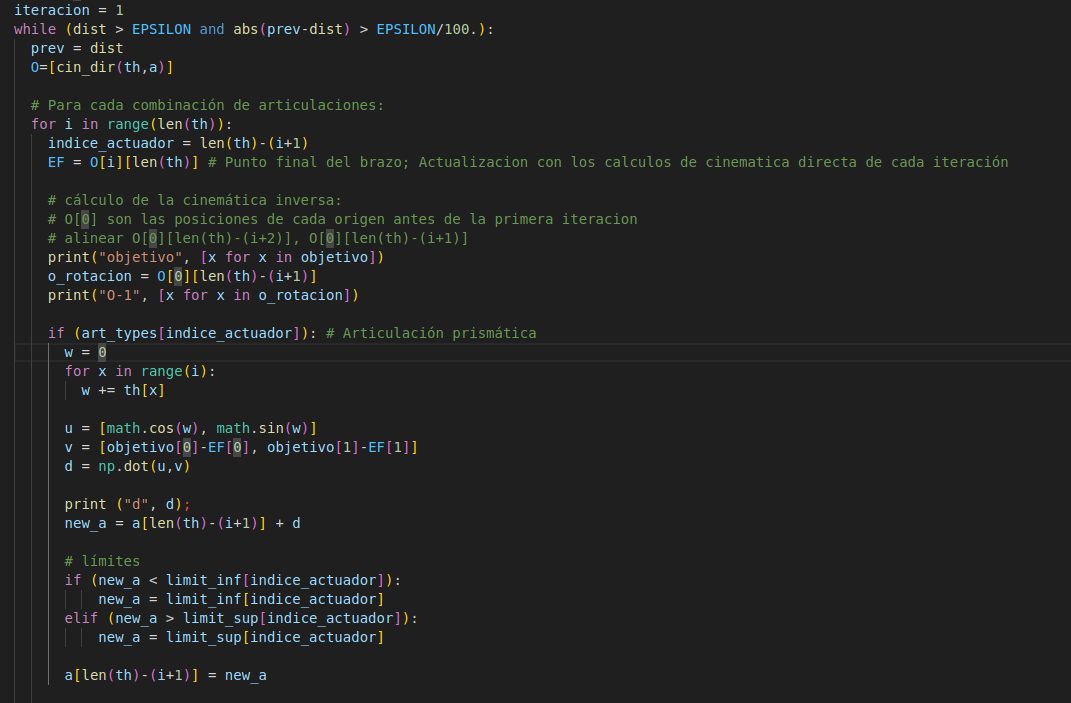
\includegraphics[width=1\linewidth]{images/ccd_1.png}
   \caption{Código del CCD para articulaciones prismáticas}
   \label{chapter:code_ccd1}
\end{figure}
\begin{figure}[htb]
   \centering
   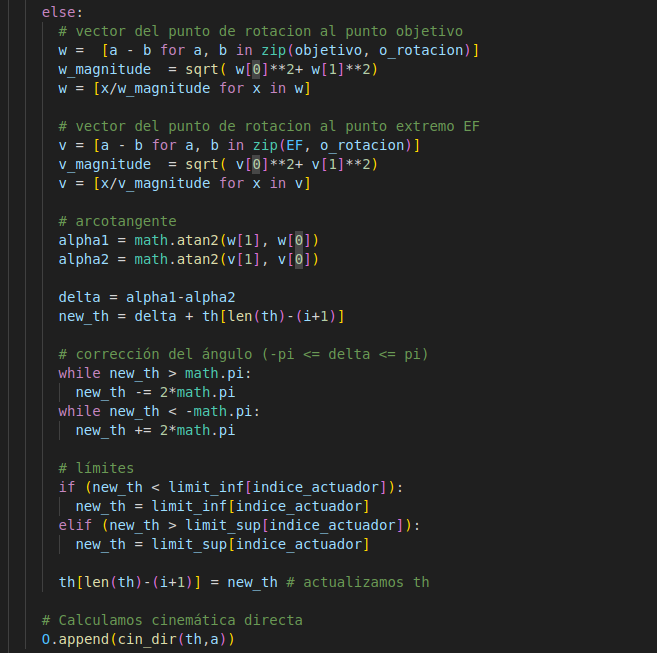
\includegraphics[width=1\linewidth]{images/ccd_2.png}
   \caption{Código del CCD para articulaciones de revolución}
   \label{chapter:code_ccd2}
\end{figure}

\subsection{Complejidad}
Para la cinemática inversa, se realiza una aproximación iterativa, en la que en cada iteración se debe calcular cada articulación.
Tras actualizar cada articulación, se debe recalcular la cinemática directa.
Es decir, para N articulaciones en una iteración se debe calcular N veces la cinemática directa. Como se dijo en el anterior capítulo, la cinemática directa es lineal respecto al número de articulaciones, por lo que la complejidad de la cinemática inversa es cuadrática $\sim O(N^2) $.

\subsection{Fé de erratas}
El código entregado en prácticas contenía un pequeño pero importante error. En la detección del tipo de articulación, se estaba empleando un índice incorrecto: se recorría en el orden inverso, de origen a extremo. Esto provocaba que se detectaran las articulaciones de forma incorrecta. No se había detectado en la entrega ya que los ejemplos provados eran simétricos en ese sentido. Se ha corregido este problema, y como se puede observar más adelante, el programa funciona correctamente en todos los casos.

%%%%%%%%%%%%%%%%%%%%%%%%%%%%%%%%%%%%%%%%%%%%%%%%%%%%%%%%%%%%%


\section{Mejoras}
Se ha implementado una sola mejora, la lectura de JSON.

\subsection{Lectura de JSON}
Se leen las características de cada articulación desde un fichero JSON. Cada articulación se caracteriza por su tipo (rotacion o primastica), sus parámetros de Denavit-Hartenberg (th y a),
y sus límites inferiores y superiores, expresados en unidades de longitud o radianes.

En el fichero, las articulaciones se indican en orden desde el origen hasta el extremo, siendo la primera la más cercana al origen.

En la figura \ref{chapter:code_ccd3} se muestra el código implementado para la lectura de JSON. En la figura \ref{chapter:ccd_json1} se observa un ejemplo de fichero JSON para un robot con una articulación de rotación, otra prismática, y otra de revolución.
\begin{figure}[htb]
   \centering
   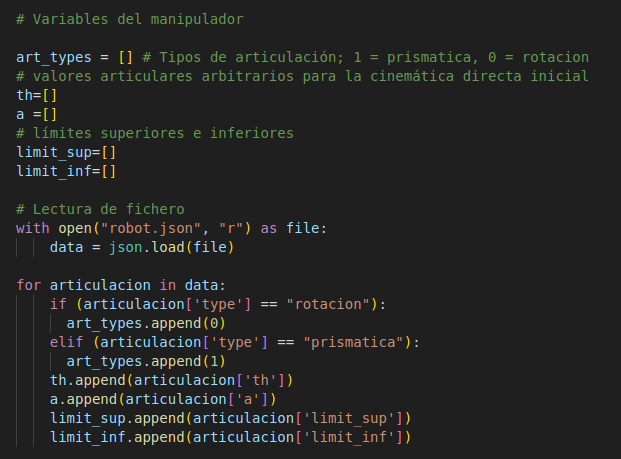
\includegraphics[width=.8\linewidth]{images/ccd_3.png}
   \caption{Código para la lectura de JSON}
   \label{chapter:code_ccd3}
\end{figure}
\begin{figure}[htb]
   \centering
   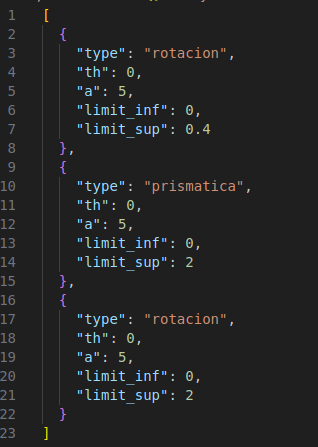
\includegraphics[width=.4\linewidth]{images/ccd_json1.png}
   \caption{Ejemplo de fichero JSON para un robot de 3 articulaciones}
   \label{chapter:ccd_json1}
\end{figure}


\subsection{Propuestas}
Actualmente solo se consideran las dimensiones iniciales del robot para la visualización. Sería interesante considerar también las coordenadas del punto objetivo para garantizar que se visualiza correctamente.
%%%%%%%%%%%%%%%%%%%%%%%%%%%%%%%%%%%%%%%%%%%%%%%%%%%%%%%%%

\section{Ejemplo}
En la figura \ref{chapter:ccd_json2} se muestra un ejemplo de fichero JSON con las características de un robot de 5 articulaciones.
\begin{figure}[htb]
   \centering
   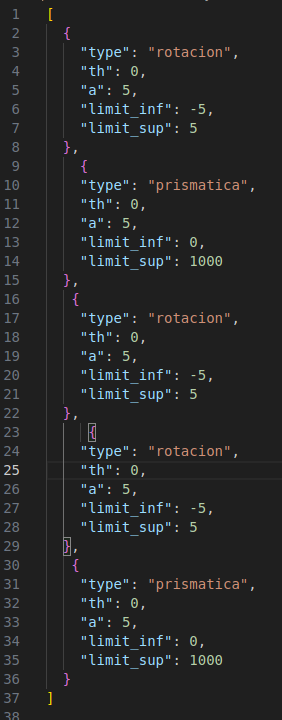
\includegraphics[width=.4\linewidth]{images/ccd_json2.png}
   \caption{Ejemplo de fichero JSON para un robot de 5 articulaciones}
   \label{chapter:ccd_json2}
\end{figure}

\subsection{Ejecución 1}
En la figura \ref{chapter:ccd_ejemplo1} se muestra la primera iteración del algoritmo sobre el robot descrito considerando como objetivo el punto 10,10.
En la figura \ref{chapter:ccd_ejemplo2} se muestra la última iteración del algoritmo, en la que se ha alcanzado el umbral de convergencia. En este caso, se consigue converger en solo 2 iteraciones.

\begin{figure}[htb]
   \centering
   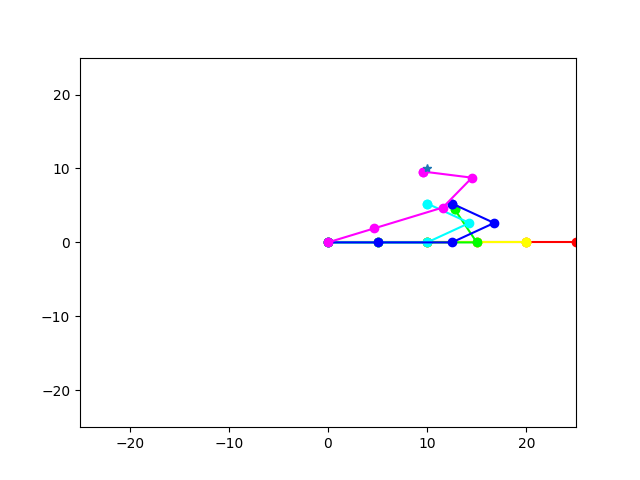
\includegraphics[width=.8\linewidth]{images/ccd_5.png}
   \caption{Primera iteración para objetivo 10,10}
   \label{chapter:ccd_ejemplo1}
\end{figure}
\begin{figure}[htb]
   \centering
   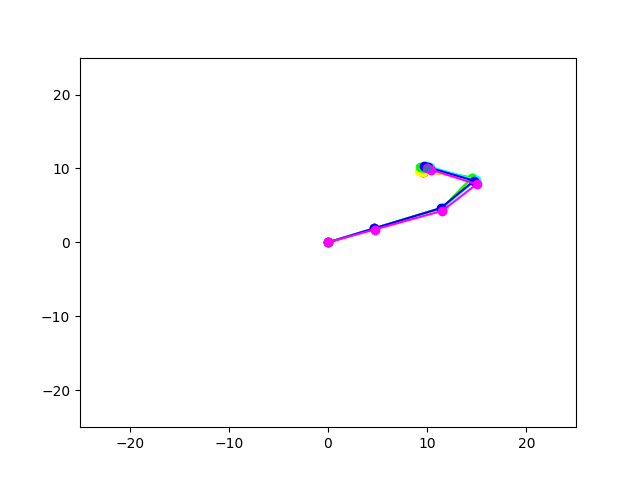
\includegraphics[width=.8\linewidth]{images/ccd_6.png}
   \caption{Última iteración para objetivo 10,10}
   \label{chapter:ccd_ejemplo2}
\end{figure}

\subsection{Ejecución 2}
En la figura \ref{chapter:ccd_ejemplo3} se muestra la primera iteración del algoritmo sobre el robot descrito considerando como objetivo el punto -20,-20.
En la figura \ref{chapter:ccd_ejemplo4} se muestra la última iteración del algoritmo, en la que se ha alcanzado el umbral de convergencia. En este caso, se consigue converger en 5 iteraciones.

\begin{figure}[htb]
   \centering
   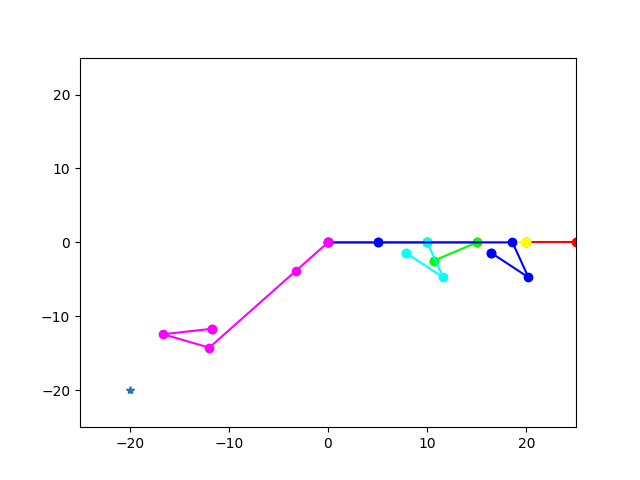
\includegraphics[width=.8\linewidth]{images/ccd_7.png}
   \caption{Primera iteración para objetivo -20,-20}
   \label{chapter:ccd_ejemplo3}
\end{figure}
\begin{figure}[htb]
   \centering
   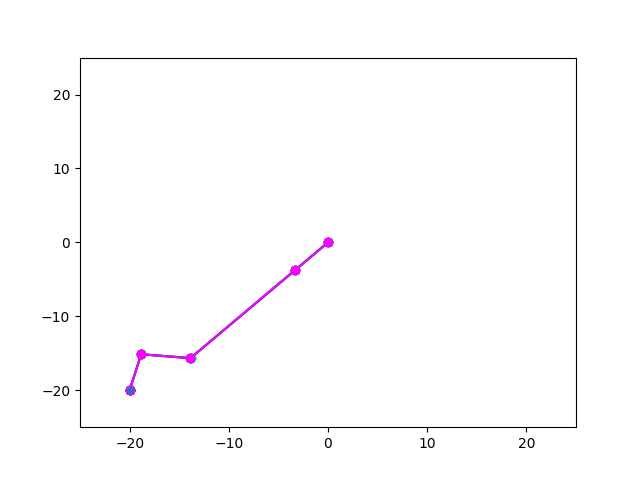
\includegraphics[width=.8\linewidth]{images/ccd_9.png}
   \caption{Última iteración para objetivo -20,-20}
   \label{chapter:ccd_ejemplo4}
\end{figure}


\subsection{Ejecución 3}
Empleando el robot de la figura \ref{chapter:ccd_json1} se comprueba que se detectan los casos en los que no se converge, esto es, no existe solución para alcanzar el punto objetivo con el robot dado.

La figura \ref{chapter:ccd_ejemplo5} muestra la última iteración para el punto objetivo 10,10. Por los límites establecidos, el robot solo puede alcanzar puntos a un radio de 12 unidades, por lo que no puede llegar al punto 10,10.
En la figura \ref{chapter:ccd_ejemplo6} se muestra la salida por consola indicando que no se ha podido converger, ya que se detecta que la distancia al objetivo ha disminuido menos de epsilon/100.
\begin{figure}[htb]
   \centering
   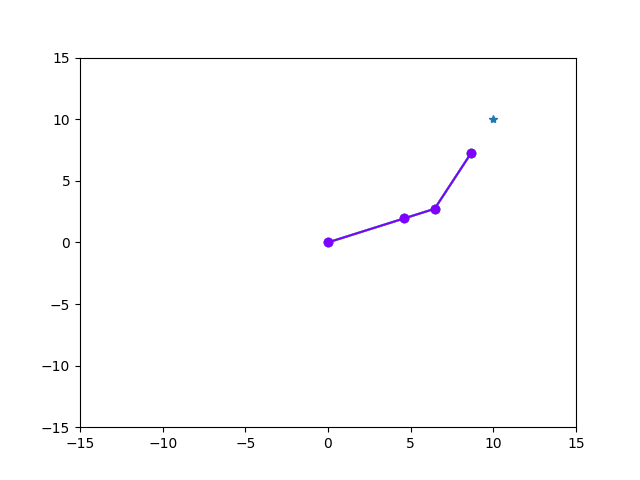
\includegraphics[width=.8\linewidth]{images/ccd_10.png}
   \caption{Última iteración para objetivo 10,10}
   \label{chapter:ccd_ejemplo5}
\end{figure}
\begin{figure}[htb]
   \centering
   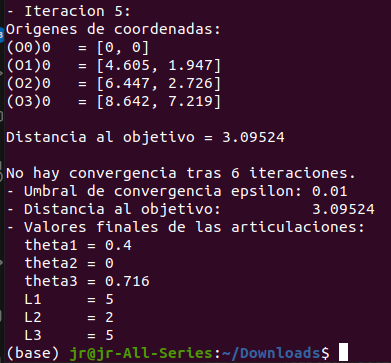
\includegraphics[width=.6\linewidth]{images/ccd_11.png}
   \caption{Salida por consola cuando no converge}
   \label{chapter:ccd_ejemplo6}
\end{figure}


\section{Conclusions}

Umbral de convergencia

%%%%%%%%%%%%%%%%%%%%%%%%%%%%%%%%%%%%%%%%%%%%%%%%%%%%%%%%%
\newpage{\pagestyle{empty}}
\thispagestyle{empty}

\chapter{\LARGE Localización}
\label{chapter:cuatro}

En esta práctica se aborda el problema de localización de un robot móvil. Se considera un robot con un sistema sensor, que tiene un cierto error de medición, y unas balizas, que son los puntos respecto a los que se toman las mediciones. 
En este caso, las balizas son a la vez los objetivos, es decir, describen la ruta que debe seguir el robot. Para esta simulación se calcula la predicción o modelo de la posición del robot, en base al movimiento que se realiza en los actuadores. 
No obstante, este movimiento tiene un cierto ruido, por lo que la posición real del robot dista de la posición ideal o estimada. Por tanto, se deben emplear las mediciones para corregir el modelo y ajustarlo a la realidad.


\section{Código Implementado}
El script proporcionado contiene muchas de las funciones necesarias, sin embargo, se debe implementar código para poder calcular la localización.

\subsection{Análisis}
Se implementan las siguientes características:
\begin{itemize}
  \item \texttt{Función de localización}: Dadas las balizas, el robot ideal, el robot real y las mediciones, se toma un punto de búsqueda a partir del cual se explora un área cuadrada comprendida entre -radio y radio, 
  usando un incremento indicado como parámetro. Se comprueban todas las posiciones posibles dentro de ese área, y se calcula la probabilidad de cada una en función de las mediciones del sensor y las posiciones de las balizas.
  Por último, se devuelve la posición con mayor probabilidad. Esta función se puede observar en la figura \ref{fig:localizacion_fun1}.
  \item \texttt{Localización inicial}: Para comenzar la localización, se debe determinar la posición en la que comienza el robot. \ref{fig:localizacion_inicial}.
  \item \texttt{Ajuste de la posición}: Mientras el robot se mueve, se debe verificar si la posición predicha es correcta, para ello se comprueba la probabilidad de las mediciones de los sensores respecto a la posición predicha.
  Se establece un umbral de error, que al ser superado causa un ajuste de la posición del modelo. Para ello, se emplea la función de localización descrita, tomando un radio de $2*error\_mediciones$. \ref{fig:localizacion_correccion}.
\end{itemize}

En la figura \ref{fig:localizacion_param} se observan algunos de los parámetros que se han indicado del script, más adelante se experimentará con ellos. 

\begin{figure}[htb]
  \centering
  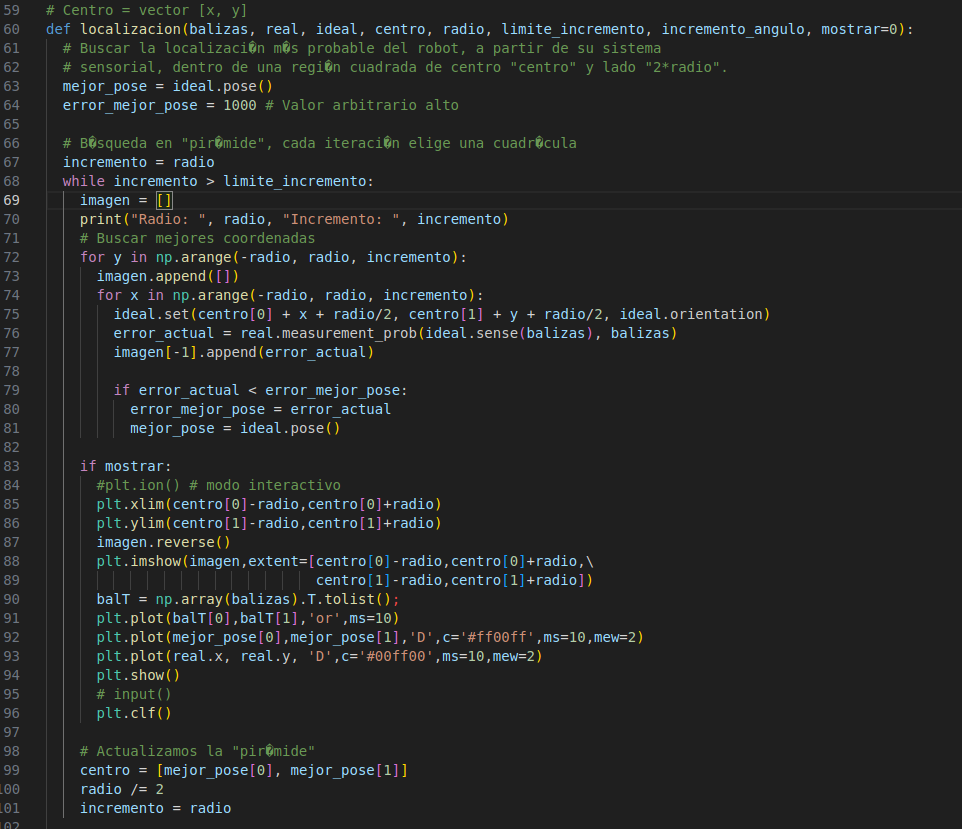
\includegraphics[width=1\linewidth]{images/localizacion1.png}
  \caption{Primera parte de la función de localización}
  \label{fig:localizacion_fun1}
\end{figure}
\begin{figure}[htb]
  \centering
  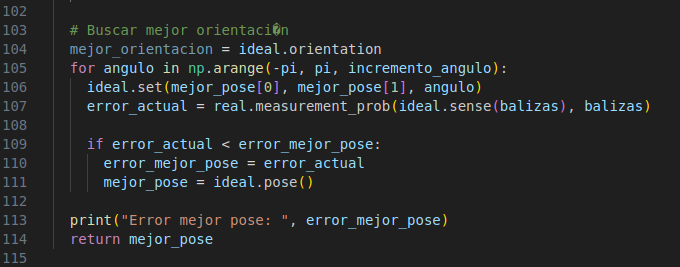
\includegraphics[width=.8\linewidth]{images/localizacion2.png}
  \caption{Fin de la función de localización}
  \label{fig:localizacion_fun2}
\end{figure}
\begin{figure}[htb]
  \centering
  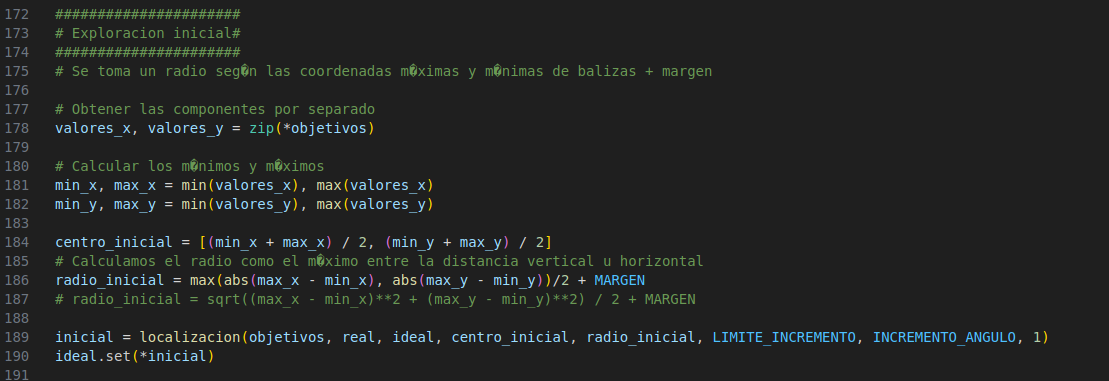
\includegraphics[width=1\linewidth]{images/localizacion5.png}
  \caption{Localización inical}
  \label{fig:localizacion_inicial}
\end{figure}
\begin{figure}[htb]
  \centering
  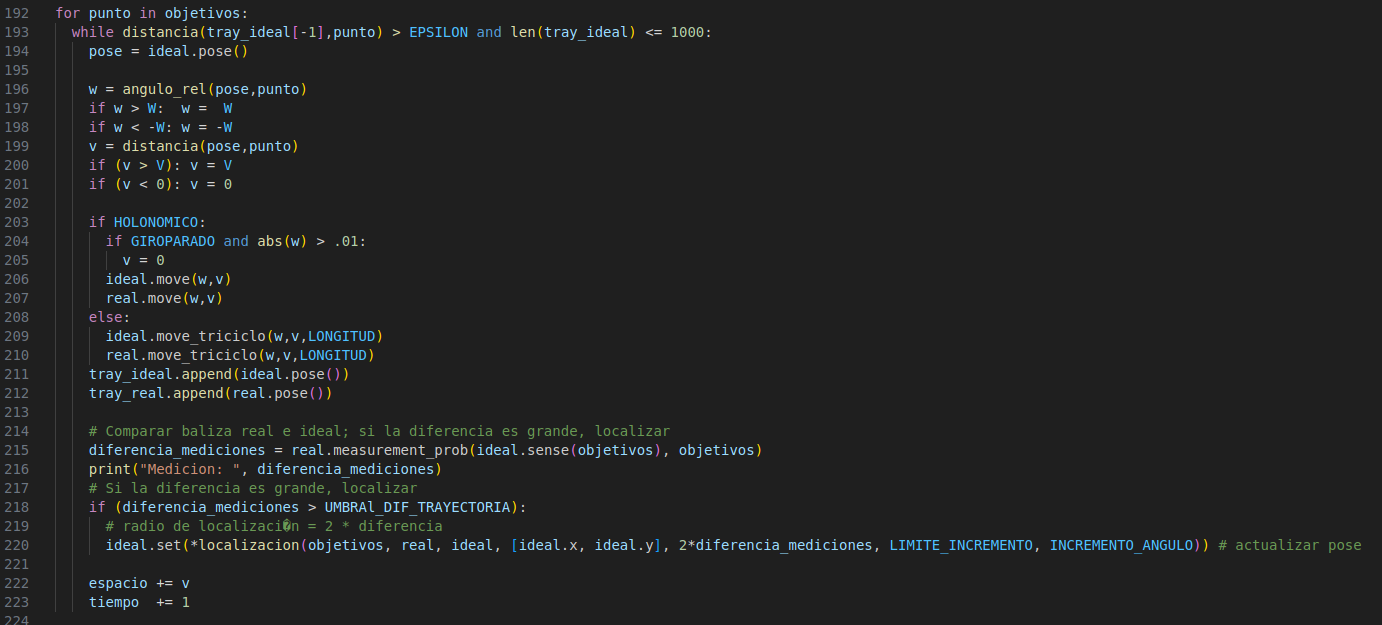
\includegraphics[width=1\linewidth]{images/localizacion6.png}
  \caption{Corrección de la posición}
  \label{fig:localizacion_correccion}
\end{figure}
\begin{figure}[htb]
  \centering
  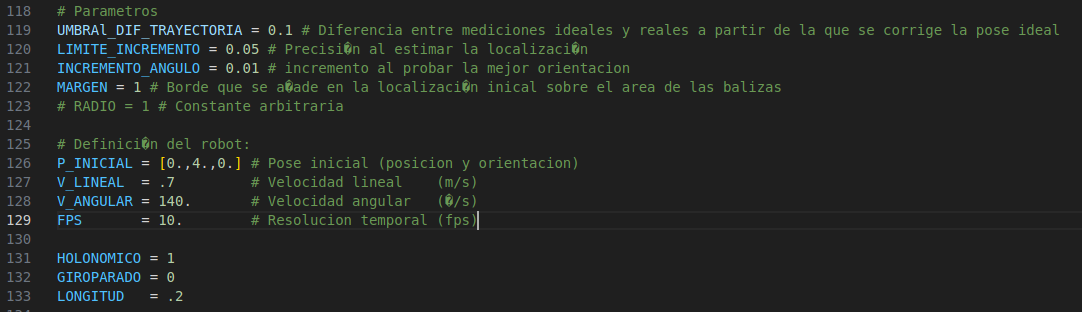
\includegraphics[width=1\linewidth]{images/localizacion3.png}
  \caption{Parámetros de la localización}
  \label{fig:localizacion_param}
\end{figure}

\subsection{Complejidad}
Los cálculos del algoritmo de localización se deben realizar al inicio, y luego cuando se supera el umbral de error. Por tanto, el rendimiento del programa dependerá del ruido en el movimiento, así como del ruido de los sensores, 
y principalmente, del umbral de error considerado. Un mayor umbral resulta en menos cálculos, mientras que un umbral menor requiere una mayor precisión, y por tanto, más cálculos. Se debe tener cuidado, puesto que un umbral demasiado bajo 
puede causar cálculos excesivos debido a los ruidos de sensores.

\bigskip Respecto a la función de localización, su complejidad depende del radio y el incremento considerado. Un menor incremento realiza un barrido más exhaustivo del área, pero requiere más cálculos. Por tanto, es importante elegir un valor que 
consiga un balance entre precisión y rendimiento.

%%%%%%%%%%%%%%%%%%%%%%%%%%%%%%%%%%%%%%%%%%%%%%%%%%%%%%%%%%%%%

\section{Mejoras}
En adición al comportamiento básico, se han implementado varias mejoras:
\subsection{Ajuste de la orientación} Además del ajuste de la posición, se implementa un cálculo similar para detectar la orientación (rotación) más probable. Se realiza un barrido entre $-\pi$ y $\pi$ con un incremento dependiente de un parámetro, y se calcula la probabilidad de cada orientación en función de las mediciones y la posición previamente predicha. El código correspondiente se aprecia en la figura \ref{fig:localizacion_fun2}.
\subsection{Uso de incremento piramidal} En lugar del comportamiento descrito previamente, en el que se emplea un incremento constante para el barrido del área a estudiar, se emplea un algoritmo de barrido piramidal, en el que en cada iteración se divide el área en 4 cuadrantes,
estudiándose el centro de cada uno, y seleccionando el cuadrante con mayor probabilidad. Este proceso se repite hasta que los cuadrantes tienen un tamaño inferior a un límite establecido. El código correspondiente se muestra en la figura \ref{fig:localizacion_fun1}. Cabe destacar
que esta forma es mucho más eficiente para estudiar el área, puesto que se evitan cálculos innecesarios. Sin embargo, se puede perder un poco de precisión ya que es posible que se seleccione un cuadrante erróneo si el punto se sitúa en el extremo entre dos, debido a los ruidos.
\subsection{Cálculo de un radio inicial en función de las balizas y margen} La alternativa inicial consiste en establecer un radio arbitrario para el primer barrido. En su lugar,
se decide implementar un cálculo del cuadrado que contiene a las balizas, mediante la selección de los mínimos y máximos de las componentes de sus coordenadas. A este área se le suma un cierto márgen
en el que puede encontrarse el robot. De esta forma se consigue una aproximación más precisa en función de la geometría de las balizas.
\subsection{Propuestas}
En adición a las mejoras implementadas, se proponen las siguientes:
\begin{itemize}
  \item \texttt{Lectura de los datos de configuración desde un JSON}: Actualmente los parámetros se encuentran en el propio script, lo que dificulta su modificación. Se propone implementar un archivo JSON en el que se almacenen los parámetros, de forma que se puedan modificar sin necesidad de acceder al código.
  \item \texttt{Visualización de múltiples trayectorias en una misma ejecución}: Sería valioso poder comparar varias trayectorias, ya sea de distintas ejecuciones con los mismos parámetros, debido a los ruidos, o para comparar distintas configuraciones.
\end{itemize}
%%%%%%%%%%%%%%%%%%%%%%%%%%%%%%%%%%%%%%%%%%%%%%%%%%%%%%%%%%%%%
\section{Ejemplos de ejecución}
\subsection{Ejemplo 1}
Se estudia la ejecución para un caso de 4 balizas, con un límite de incremento para la localización de 0.05 y un umbral para la corrección de trayectoria de 0.1. El resto de parámetros se mantienen en sus valores por defecto.

\bigskip En primer lugar analizamos al localización inicial. En la figura \ref{fig:localizacion_ej1} se observa la primera iteración. Se distinguen los 4 cuadrantes y se muestra en tonos morados el que tiene mayor probabilidad.
Además, se observa la posición real del robot con un diamante verde, y la posición estimada, que corresponde con el centro del cuadrante, con un diamante violeta.
A continuación, en la figura \ref{fig:localizacion_ej2} se muestra la última iteración, en la que se observa que la posición estimada está bastante cerca de la real, (4.0625, -0.0650) vs (4.0, 0.0) respectivamente. Además observamos que en esta iteración la probabilidad de los centros de los cuadrantes es menor que la de probabilidad de la iteración previa, por lo que la posición estimada se mantiene sin cambios.
\begin{figure}[htb]
  \centering
  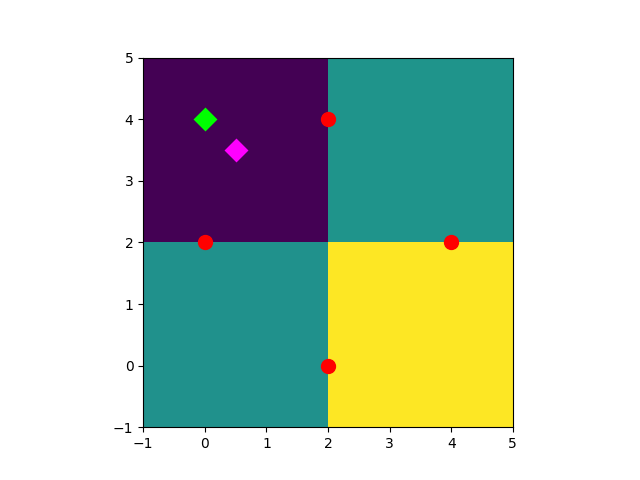
\includegraphics[width=1\linewidth]{images/localizacion7.png}
  \caption{Primera iteración de la localización inicial}
  \label{fig:localizacion_ej1}
\end{figure}
\begin{figure}[htb]
  \centering
  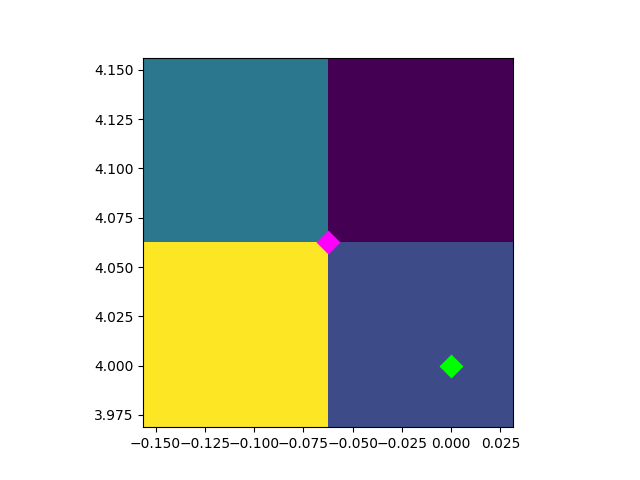
\includegraphics[width=1\linewidth]{images/localizacion8.png}
  \caption{Última iteración de la localización inicial}
  \label{fig:localizacion_ej2}
\end{figure}

\bigskip En la figura \ref{fig:localizacion_ej3} se observa la evolución de la posición real del robot en rojo, así como las correcciones de la posición ideal, en verde. Vemos como cuando la trayectoria predicha se separa lo suficiente de la real, se realiza una corrección.

\begin{figure}[htb]
  \centering
  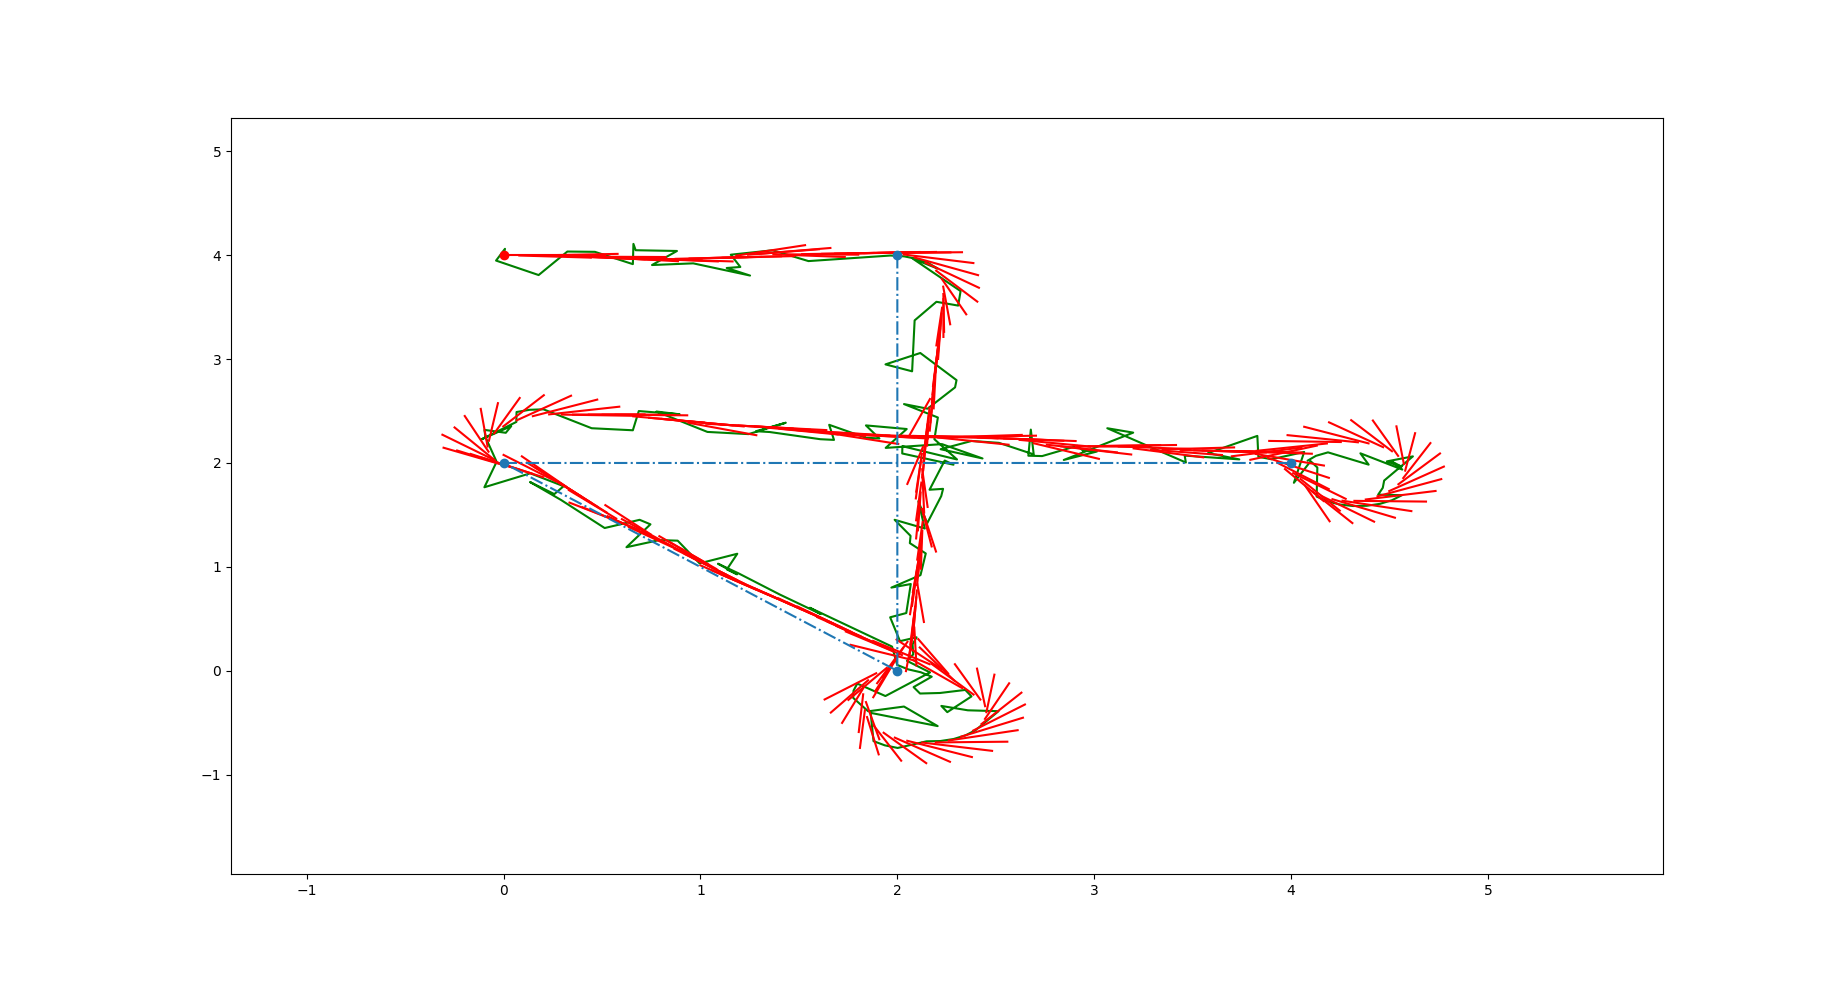
\includegraphics[width=1\linewidth]{images/localizacion9.png}
  \caption{Trayectoria del ejemplo 1}
  \label{fig:localizacion_ej3}
\end{figure}

\subsection{Ejemplo 2}
Mantenemos los valores del experimento anterior, pero disminuimos el umbral a 0.01, lo que debería aumentar la precisión de la trayectoria ideal. En la figura \ref{fig:localizacion_ej4} observamos el resultado de ejecución. Cabe destacar que se han realizado giros alrededor de todas las balizas, incluso varios en el caso de la baliza izquierda. Esto 
es debido a que la trayectoria predicha se ha quedado a una distancia mayor al umbral de las balizas, por lo que se ha tenido que ajustar la trayectoria real para aseguarse de que pasa por las balizas. Además, observamos que la trayectoria ideal, en verde, se reajusta más veces que en el ejemplo 1.
\begin{figure}[htb]
  \centering
  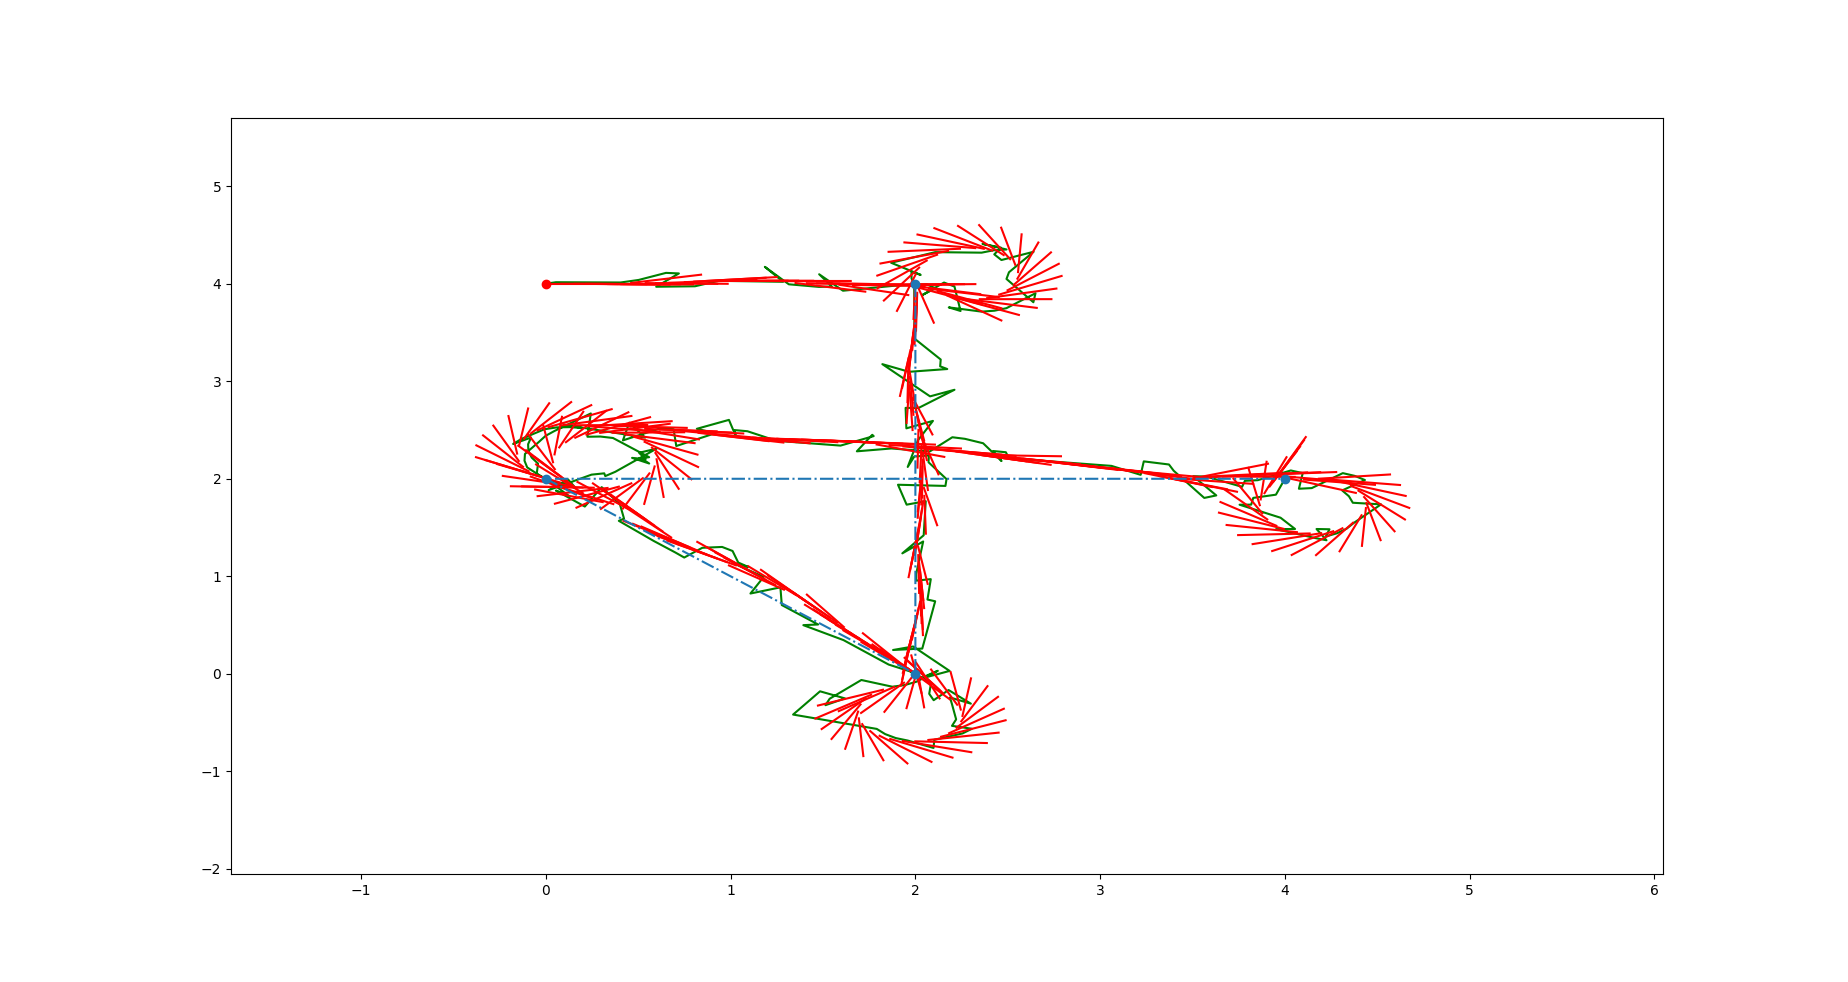
\includegraphics[width=1\linewidth]{images/localizacion10.png}
  \caption{Trayectoria del ejemplo 2}
  \label{fig:localizacion_ej4}
\end{figure}

\subsection{Ejemplo 3}
Ahora consideramos la configuración del ejemplo 2, pero aumentamos la velocidad angular a 240º por segundo (por defecto estaba a 140º/s). 
En la figura \ref{fig:localizacion_ej5} se observa la trayectoria del robot. Constatamos que los giros son más cerrados.

\begin{figure}[htb]
  \centering
  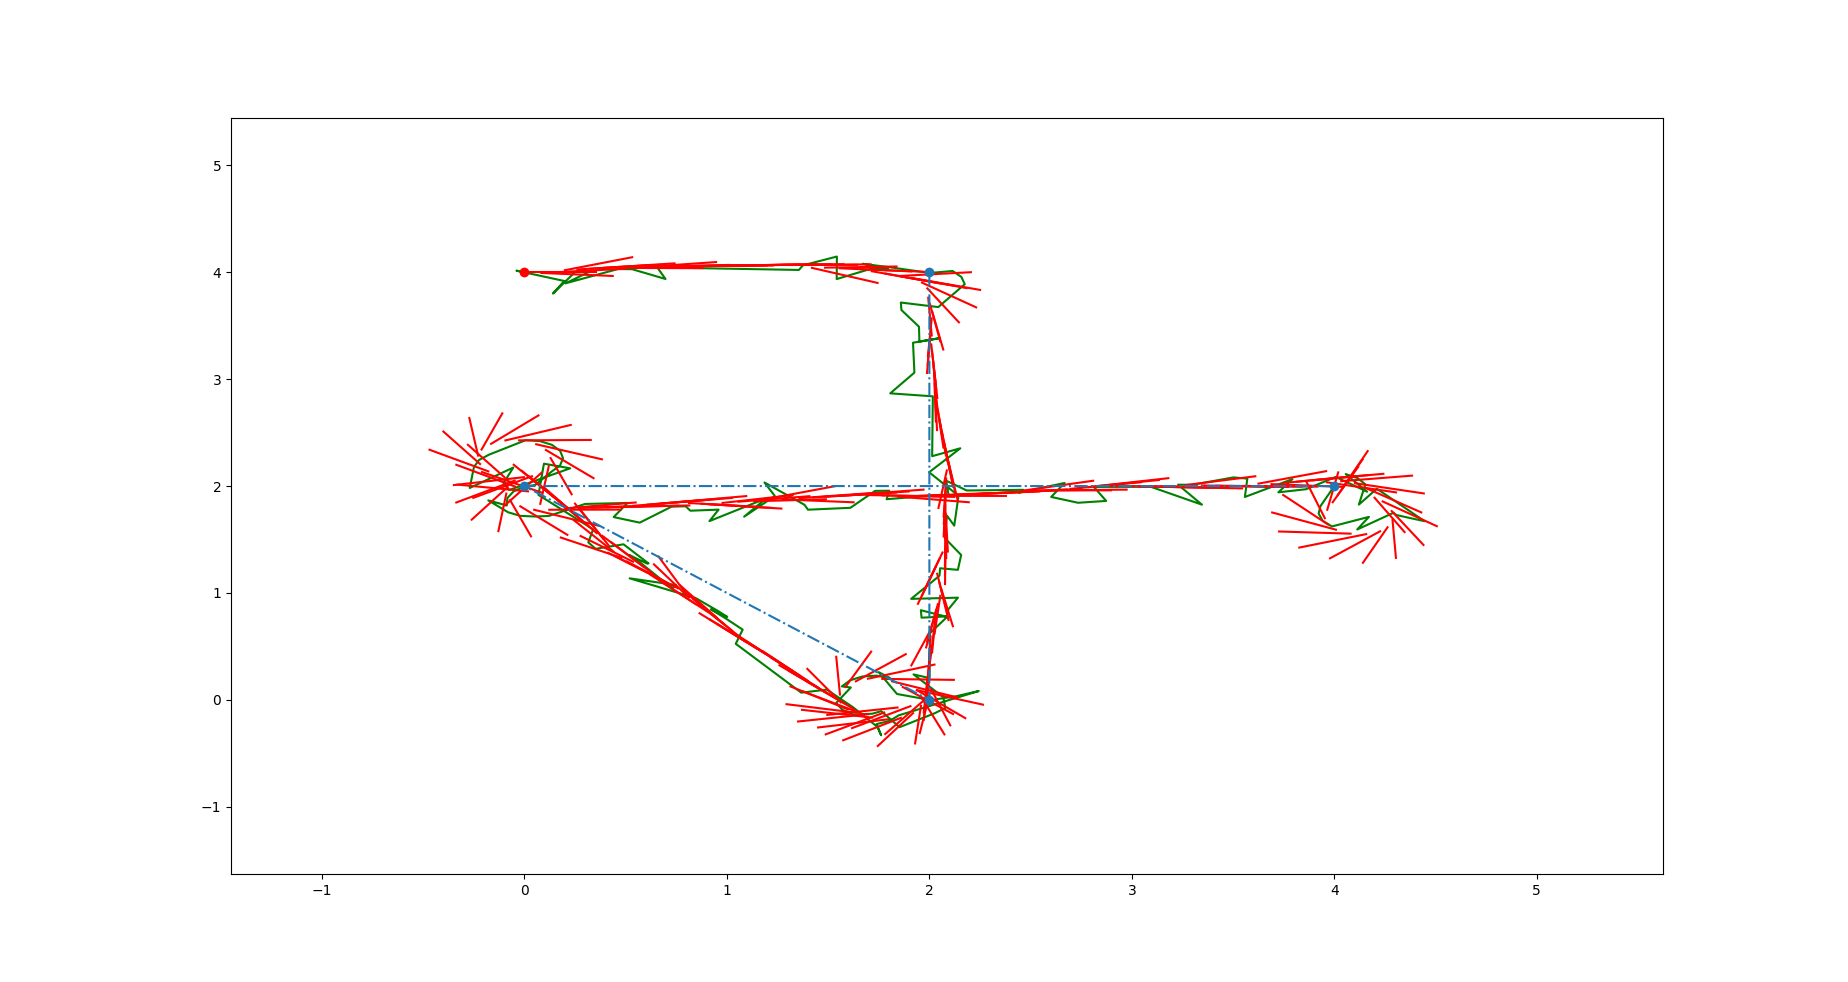
\includegraphics[width=1\linewidth]{images/localizacion11.png}
  \caption{Trayectoria del ejemplo 3}
  \label{fig:localizacion_ej5}
\end{figure}

\subsection{Ejemplo 4}
En este caso mantenemos los valores del ejemplo 2, pero reducimos la velocidad angular a 40º por segundo. 
En la figura \ref{fig:localizacion_ej6} se observa la trayectoria del robot. Vemos que ahora los giros son más abiertos, y en consecuencia, el robot tarda más
en realizar el recorrido y requiere computar más posiciones.

\begin{figure}[htb]
  \centering
  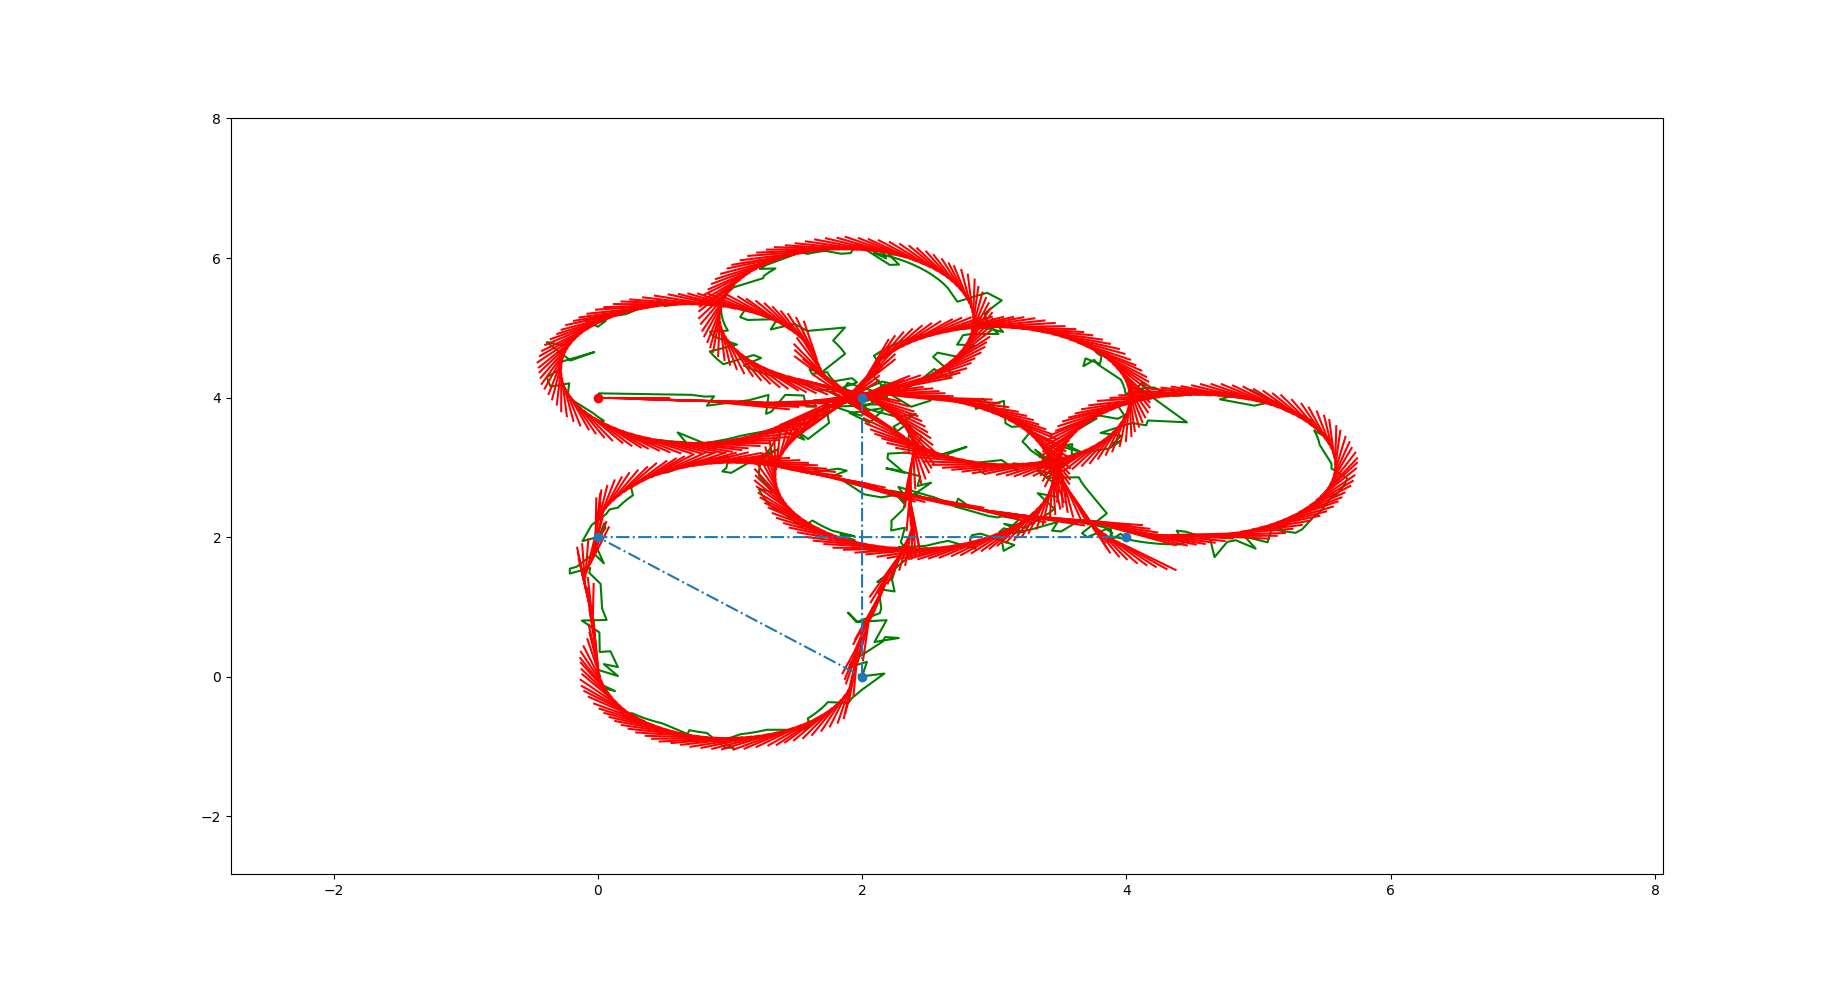
\includegraphics[width=1\linewidth]{images/localizacion12.png}
  \caption{Trayectoria del ejemplo 4}
  \label{fig:localizacion_ej6}
\end{figure}

%%%%%%%%%%%%%%%%%%%%%%%%%%%%%%%%%%%%%%%%%%%%%%%%%%%%%%%%%%%%%
\section{Conclusions}
We have implemented an algorithm for modelling the position and orientation (the pose) of a mobile robot, considering the predicted pose and making adjustments based on sensor measurements regarding the position of beacons.
We have made improvements such as using a variable increment for the search area through a pyramidal approach.

\bigskip Also, we have considered the complexity of the algorithm, which depends on the noise in the movement and sensors, as well as the threshold for the error. A lower threshold requires more calculations, so it is important to find a balance between precision and performance.
This has been proved experimentally. Additionally, we have also tested the impact of the angular velocity on the robot's trajectory, seen that a higher angular velocity results in tighter turns whereas a lower angular velocity results in wider turns and usually a longer trajectory.

\bigskip Althoug the algorithm has performed well on the experiments, it has a relatively high computational cost, and a more efficient approach will be discussed in the next chapter, the particle filter.


%%%%%%%%%%%%%%%%%%%%%%%%%%%%%%%%%%%%%%%%%%%%%%%%%%%%%%%%%
\newpage{\pagestyle{empty}}
\thispagestyle{empty}

\chapter{\LARGE Filtro de Partículas}
\label{chapter:cinco}

En esta práctica se aborda el filtro de partículas. Se trata de un algoritmo eficiente para calcular la localización de un robot móvil que dispone de sensores de distancia.

\section{Código Implementado}
El algoritmo se basa en la generación de una serie de partículas empleando como centro la posición ideal (posición estimada) y siguiendo una distribución de probabilidad
sobre un radio indicado como parámetro. Sobre esta distribución inicial, iterativamente se aplica el movimiento del robot y se actualiza la probabilidad de cada partícula, 
tras lo que se realiza un remuestreo, en el que se escogen las partículas con mayor probabilidad.


\subsection{Análisis}
El código proporcionado contiene muchas de las funciones necesarias. Para el correcto funcionamiento se implementan las siguientes funciones:
\begin{itemize}
  \item \texttt{genera\_filtro}: Se inicializa el filtro de partículas con el tamaño indicado, para ello se crea un array de robots, siendo
cada uno una partícula. Se inicializa cada partícula con un ruido arbitrario, y se asigna una posición siguiendo una distribución uniforme en el área
descrita por el centro y el radio indicados. Adicionalmente, la orientación se establece añadiendo un ruido gaussiano a la orientación ideal. Por último,
se establece la probabilidad de cada partícula en base a las mediciones y las balizas.
  \item \texttt{dispersion}: Considera la dispersión espacial de las partículas, para ello, se retorna un array conteniendo los valores mínimos y máximos de las componentes x e y de las posiciones de todas las partículas.
  \item \texttt{peso\_medio}: Se calcula el peso medio empleando la suma de todos los pesos para normalizar el de cada partícula.
\end{itemize}
Todas estas funciones se observan en las figuras \ref{fig:genera_filtro}, \ref{fig:dispersion} y \ref{fig:peso_medio}.

\begin{figure}[htb]
  \centering
  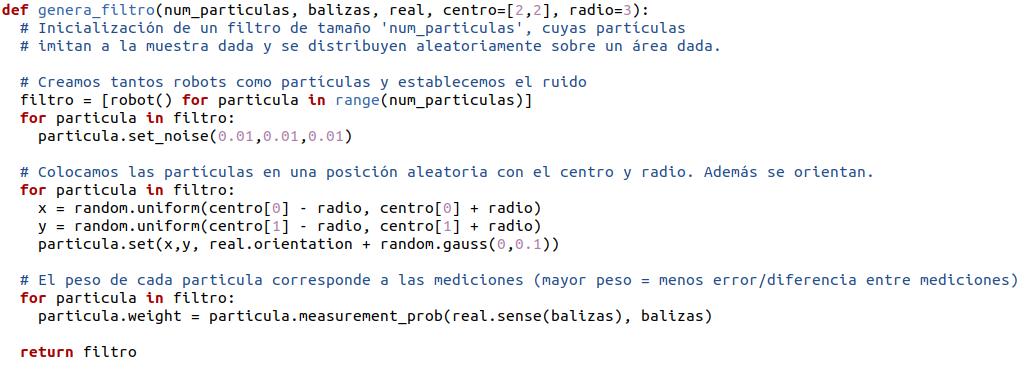
\includegraphics[width=1\linewidth]{images/filtroc1.png}
  \caption{Función \textit{genera\_filtro}}
  \label{fig:genera_filtro}
\end{figure}
\begin{figure}[htb]
  \centering
  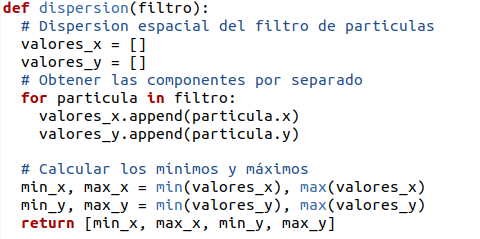
\includegraphics[width=.5\linewidth]{images/filtroc2.png}
  \caption{Función \textit{dispersion}}
  \label{fig:dispersion}
\end{figure}
\begin{figure}[htb]
  \centering
  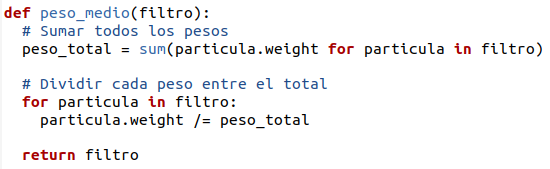
\includegraphics[width=.6\linewidth]{images/filtroc3.png}
  \caption{Función \textit{peso\_medio}}
  \label{fig:peso_medio}
\end{figure}

Además, en el programa principal se codifican los siguientes comportamientos:
\begin{itemize}
  \item \texttt{inicialización del filtro}: se crea el filtro empleando la función \textit{genera\_filtro}, usando el número de partículas inicial indicado como parámetro. Se toma además como centro la posición inical del robot, y se emplea un radio 1.
A continuación se establece como posición inicial la partícula más probable, y se inicializan la trayectoria ideal y real. El código de esta sección se muestra en la figura \ref{fig:inicializacion}.
  \item \texttt{actualización de la trayectoria y las probabilidades}: se mueven todas las partículas del filtro con el vector de movimiento calculado para dirigirse hacia el objetivo. A continuación,
se actualizan los pesos con las nuevas probabilidades, y se normalizan empleando la función \textit{peso\_medio}. Finalmente se actualiza la trayectoria real e ideal. El código de este fragmento así como 
del remuestreo se encuentra en la figura \ref{fig:actualizacion}.
  \item \texttt{remuestreo}: se emplea la función ya definida "resample", que toma como parámetros el filtro y el número de partículas deseado. 
\end{itemize}
\begin{figure}[htb]
  \centering
  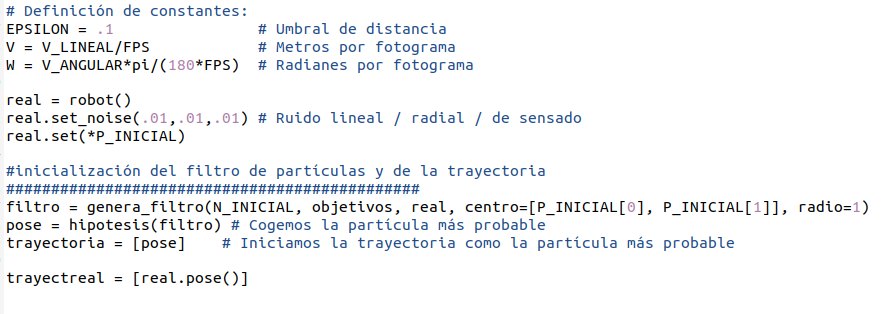
\includegraphics[width=1\linewidth]{images/filtroc4.png}
  \caption{Inicialización del filtro} 
  \label{fig:inicializacion}
\end{figure}
\begin{figure}[htb]
  \centering
  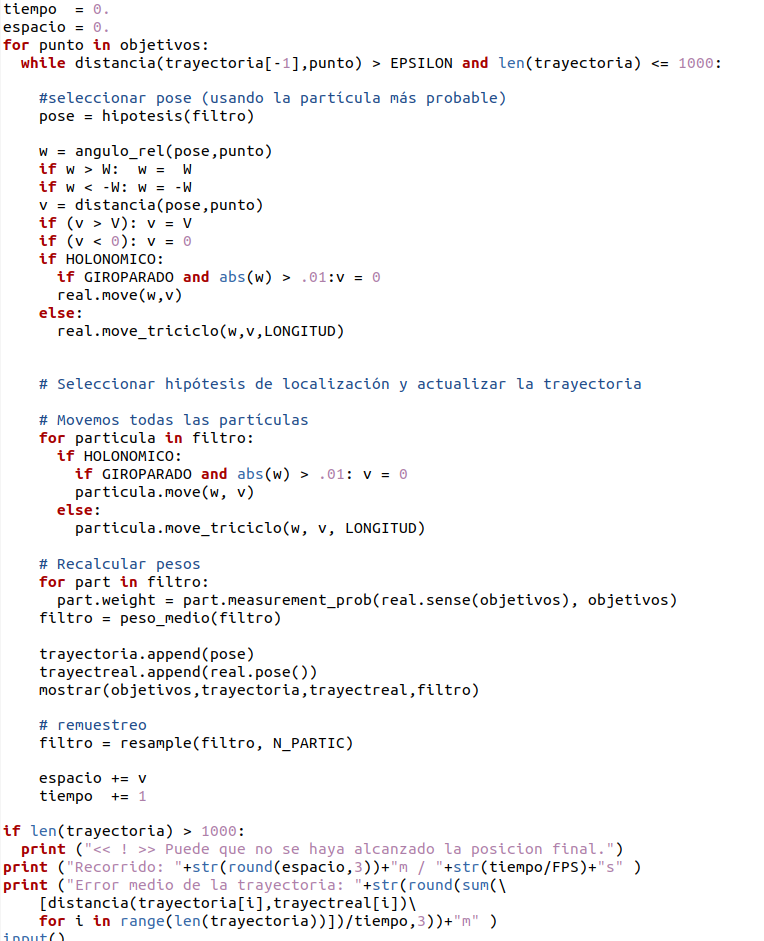
\includegraphics[width=.9\linewidth]{images/filtroc5.png}
  \caption{Actualización del filtro y remuestreo}
  \label{fig:actualizacion}
\end{figure}

\subsection{Complejidad}
El costo computacional del algoritmo depende principalmente del número de partículas que se mantienen en el filtro, el cuál es uno de los principales
parámetros a ajustar. En general, el algoritmo es lineal en el número de partículas, ya que en cada iteración se actualiza la posición y probabilidad de cada partícula.
%%%%%%%%%%%%%%%%%%%%%%%%%%%%%%%%%%%%%%%%%%%%%%%%%%%%%%%%%%%%%

\section{Mejoras}
No se han implementado mejoras, pero se proponen las siguientes:
\begin{itemize}
  \item \texttt{Número variable de partículas}: Emplear un enfoque adaptativo, en el que el número de partículas se ajuste en función
de la precisión del modelo (la probabilidad de que la posición predicha sea correcta según las mediciones).
  \item \texttt{Lectura de datos de configuración desde un JSON}: al igual que en prácticas anteriores, se podría emplear un fichero de configuración para evitar tener
que modificar el código cuando se quieren alterar parámetros como el número de partículas, el radio de dispersión, etc.
  \item \texttt{Mejoras del remuestreo}: ahora mismo se implementa un remuestreo básico, sería interesante considerar aproximaciones más inteligentes, como 
por ejemplo, remuestreo estratificado, en el que se busca mejorar la representatividad de las partículas escogidas.
\end{itemize}

%%%%%%%%%%%%%%%%%%%%%%%%%%%%%%%%%%%%%%%%%%%%%%%%%%%%%%%%%%%%%
\section{Ejemplos de ejecución}
Se han realizado varios experimentos sobre la trayectoria con 3 balizas.
\subsection{Ejemplo 1}

Realizamos una ejecución para comprobar el funcionamiento con los valores por defecto, destacando que el tamaño inicial del filtro es de 2000 partículas, y el tamaño el resto de las iteraciones es de 50.

Observamos en la figura \ref{fig:ejemplo1} el inicio del experimento, en el que se observa la posición inicial del robot y las partículas generadas. En la figura \ref{fig:ejemplo2} se muestra la segunda iteración, en la que se observa la reducción del número de partículas.
En la figura \ref{fig:ejemplo3} se muestra el progreso del experimento, destacando la existencia de tres grupos de partículas, unas por encima de la posición real, otras simétricamente por debajo, y el resto en la posición real. Esto se debe a la ambigüedad de las mediciones con la configuración de las balizas.
En la figura \ref{fig:ejemplo4} se muestra la convergencia del experimento, en la que se observa que las partículas se concentran en la posición real del robot. Por último, en la figura \ref{fig:ejemplo5} se muestra la trayectoria del robot, en la que se observa que el filtro de partículas ha sido capaz de seguir la trayectoria real del robot.

%%%%%%%%%%%%%%%%%%%%%%%%%%%
\begin{figure}[htb]
  \centering
  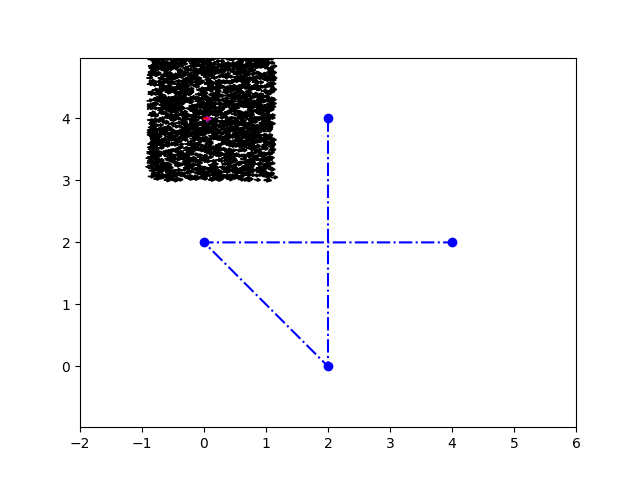
\includegraphics[width=.8\linewidth]{images/filtro1.png}
  \caption{Inicio del ejemplo 1}
  \label{fig:ejemplo1}
\end{figure}
\begin{figure}[htb]
  \centering
  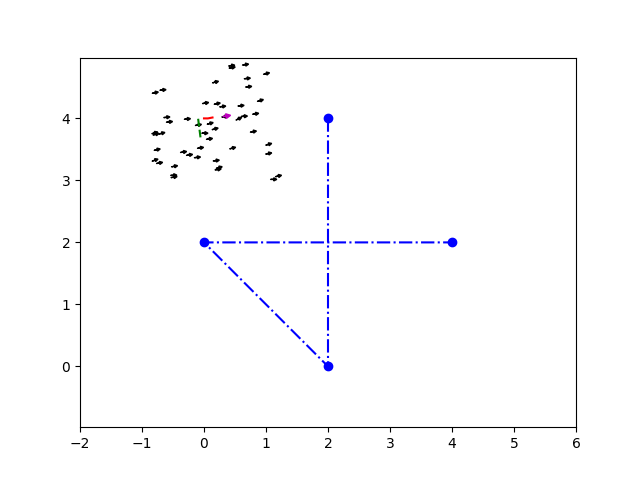
\includegraphics[width=.8\linewidth]{images/filtro2.png}
  \caption{Segunda iteración del ejemplo 1}
  \label{fig:ejemplo2}
\end{figure}
\begin{figure}[htb]
  \centering
  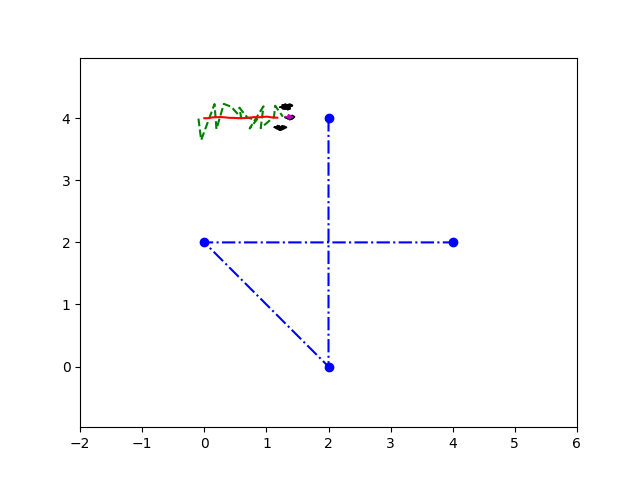
\includegraphics[width=.8\linewidth]{images/filtro3.png}
  \caption{Progreso del ejemplo 1}
  \label{fig:ejemplo3}
\end{figure}
\begin{figure}[htb]
  \centering
  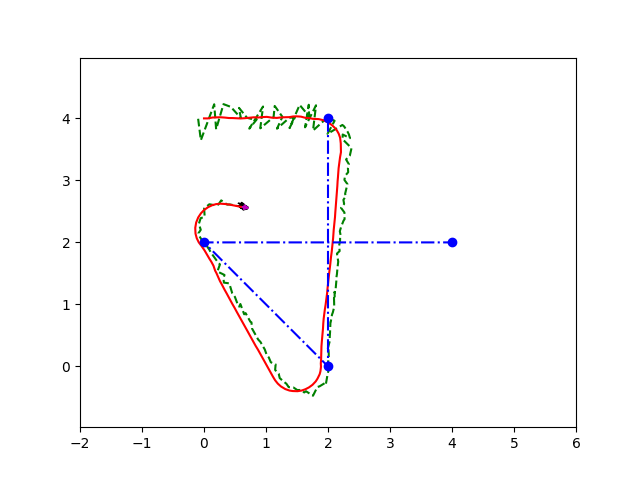
\includegraphics[width=.8\linewidth]{images/filtro4.png}
  \caption{Convergencia del ejemplo 1}
  \label{fig:ejemplo4}
\end{figure}
\begin{figure}[htb]
  \centering
  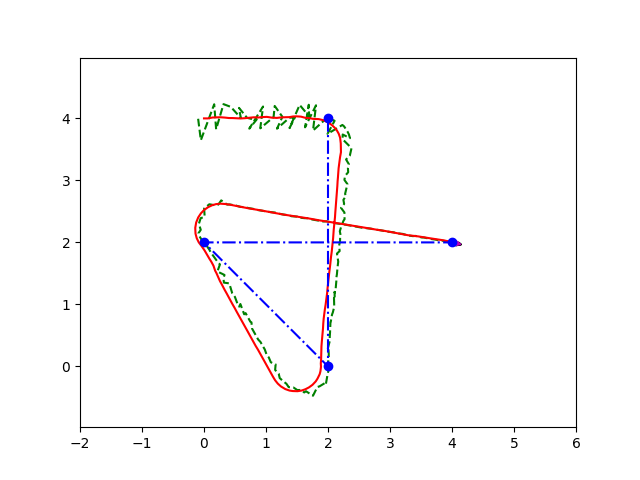
\includegraphics[width=.8\linewidth]{images/filtro5.png}
  \caption{Trayectoria del ejemplo 1}
  \label{fig:ejemplo5}
\end{figure}
%%%%%%%%%%%%%%%%%%%%%%%%%%%
\subsection{Ejemplo 2}
Se repite el experimento anterior, manteniendo el número de partículas inicial, pero con un tamaño de 100 del filtro de partículas en ejecución. En la figura \ref{fig:ejemplo7} se observa que en las primeras iteraciones ya no existe la 
ambigüedad del ejemplo previo, sino que se ve un grupo cercano de partículas. En la figura \ref{fig:ejemplo8} se observa la convergencia del experimento, que ha tenido lugar más rápido que en el anterior ejemplo. Por último, en la figura \ref{fig:ejemplo9} se muestra la trayectoria del robot, en la que se observa que el filtro de partículas ha sido capaz de seguir la trayectoria real del robot con mayor precisión, no obstante, 
cabe destacar que el coste computacional ha sido mayor, el experimento ha tardado más tiempo.
\begin{figure}[htb]
  \centering
  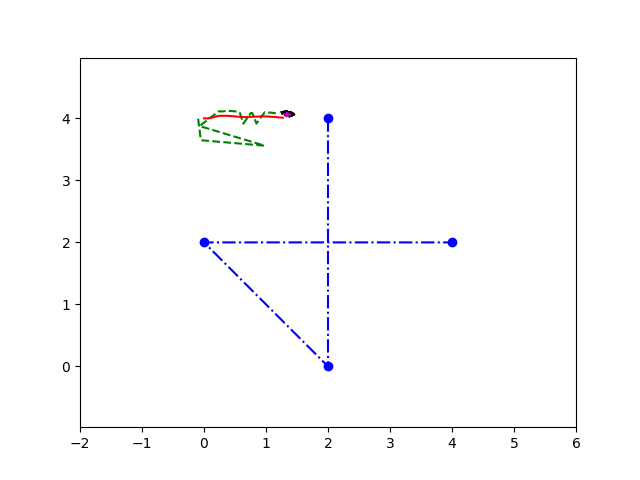
\includegraphics[width=.8\linewidth]{images/filtro7.png}
  \caption{Inicio del ejemplo 2}
  \label{fig:ejemplo7}
\end{figure}
\begin{figure}[htb]
  \centering
  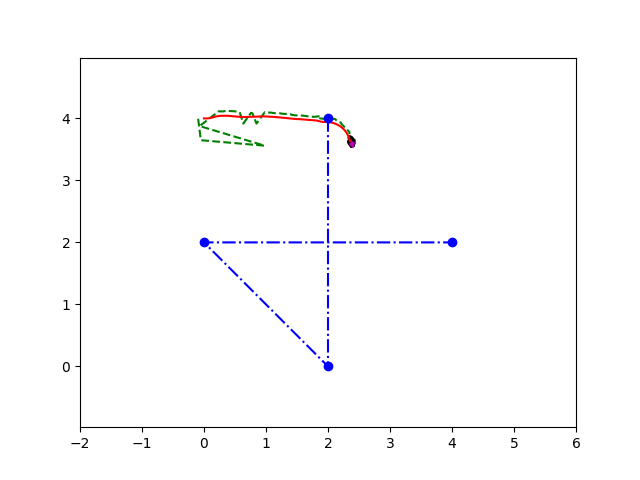
\includegraphics[width=.8\linewidth]{images/filtro8.png}
  \caption{Convergencia del ejemplo 2}
  \label{fig:ejemplo8}
\end{figure}
\begin{figure}[htb]
  \centering
  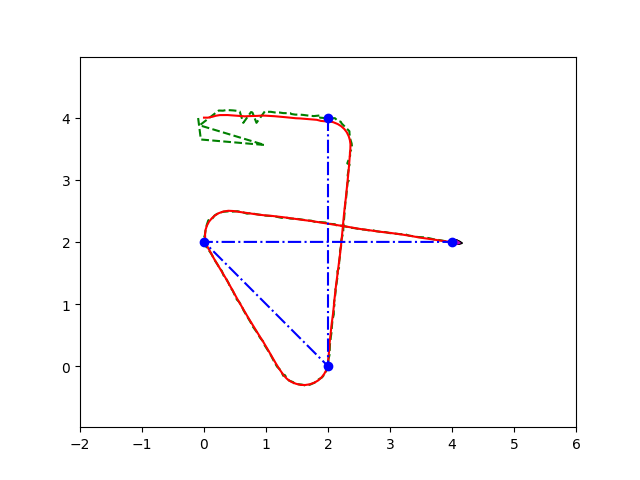
\includegraphics[width=.8\linewidth]{images/filtro9.png}
  \caption{Trayectoria del ejemplo 2}
  \label{fig:ejemplo9}
\end{figure}
%%%%%%%%%%%%%%%%%%%%%%%%%%%
\subsection{Ejemplo 3}
A continuación se repite el experimento pero para un filtro con tamaño 10.
En la figura \ref{fig:ejemplo10} se observa la trayectoria del experimento. Destaca que la precisión es mucho menor a los experimentos anteriores, y mientras que se converge rápidamente, 
se pierde la trayectoria real del robot en varias ocasiones.
\begin{figure}[htb]
  \centering
  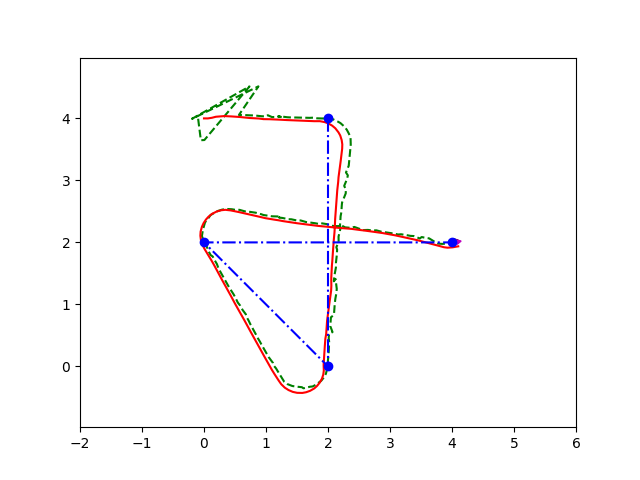
\includegraphics[width=.8\linewidth]{images/filtro10.png}
  \caption{Trayectoria del ejemplo 3}
  \label{fig:ejemplo10}
\end{figure}
%%%%%%%%%%%%%%%%%%%%%%%%%%%%%%%%%%%%%%%%%%%%%%%%%%%%%%%%%%%%%
\section{Conclusions}
We have implemented a simple particle filter and proved its functionality with some examples. We have studied the computational complexity of the algorithm and seen that
a higher particle count leads to improved precision, but also increases the computational cost. It seems that 50 particles is a good balance between precision and performance.
It is also worth noting that this algorithm is a fast approach for localization of a moving robot, being faster than the approach described in chapter 4.
%%%%%%%%%%%%%%%%%%%%%%%%%%%%%%%%%%%%%%%%%%%%%%%%%%%%%%%%%%%%%



%%%%%%%%%%%%%%%%%%%%%%%%%%%%%%%%%%%%%%%%%%%%%%%%%%%%%%%%%
\newpage{\pagestyle{empty}\cleardoublepage}
\thispagestyle{empty}

%%%%%%%%%%%%%%%%%%%%%%%%%%%%%%%%%%%%%%%%%%%%%%%%%%%%%%%%%%
% \begin{thebibliography}{X}
% % Aquí figurará la bibliografía
% \end{thebibliography}
%%%%%%%%%%%%%%%%%%%%%%%%%%%%%%%%%%%%%%%%%%%%%%%%%%%%%%%%%%

\end{document}

